% ICAMAC 2026 / IEEE Xplore proceedings draft — SyNAPSE
% Verified metrics: tests/evaluation/results/*.csv (run date 2026-09-01 UTC)
% Compile: pdflatex icamac2026_synapse.tex (twice for refs)
\documentclass[conference]{IEEEtran}
\IEEEoverridecommandlockouts
\usepackage{cite}
\usepackage{amsmath,amssymb}
\usepackage{graphicx}
\usepackage{textcomp}
\usepackage{xcolor}
\usepackage{booktabs}
\usepackage{multirow}
\usepackage{url}
\usepackage{balance}
\usepackage{tikz}
\usetikzlibrary{arrows.meta,positioning,fit,shapes.geometric}

\hyphenation{op-tical net-works semi-conduc-tor neuro-di-verse}

\begin{document}

\title{SyNAPSE: Local-First Emotion-Aware AAC with Role-Based Access and Reproducible System Benchmarks}

\author{\IEEEauthorblockN{Neha Vinod and Dr.\ Raja Varma Pamba}
\IEEEauthorblockA{\textit{Department of Computer Science and Engineering}\\
\textit{Manipal Academy of Higher Education}\\
Dubai, United Arab Emirates}}

\maketitle

\begin{abstract}
Minimally verbal neurodiverse learners depend on augmentative and alternative communication (AAC), yet most tools neither adapt vocabulary to detected affect nor coordinate teachers, caregivers, and special-education staff under strict data-minimization constraints. We present \textbf{SyNAPSE} (Symbolic Neuro-Adaptive Platform for Social Expression), a locally deployable web platform that couples on-demand facial-expression analysis (DeepFace), Ollama-hosted Llama~3 symbol generation, bilingual $4\times4$ AAC grids, WebSocket caregiver alerts, and JWT role-based access for four personas. The FastAPI/SQLite backend exposes 44 REST endpoints and two WebSocket channels; emotion logs persist labels and confidence only---no image blobs. We contribute (i)~an integrated architecture for school AAC workflows aligned with UAE inclusive-education reporting, (ii)~a reproducible evaluation harness producing CSV benchmarks, and (iii)~an explicit audit separating validated metrics from open risks. Verified results on the deployed system (2026-09-01 benchmark run): PDF generation median 0.199\,s ($n{=}30$), LLM card generation median 7.36\,s / mean 10.56\,s ($n{=}36$), WebSocket alert delivery median 0.698\,s ($n{=}30$), and LLM rule-based fallback in 22/120 trials (18.3\%, all \texttt{malformed\_json}). Role-access testing yields 100\% policy-correct outcomes (168/168) after fixing report-generation ACLs and teacher-route authorization. A FER-2013 integration pilot ($n{=}12$ crops; angry/disgust/fear only after fixture corruption) yields 41.7\% top-1 accuracy and macro-F1 0.500; legacy non-facial placeholder fixtures previously produced 0/12 accuracy (IEEE topics S4.1, S4.16, S3.18, S3.19).
\end{abstract}

\begin{IEEEkeywords}
augmentative communication, facial expression analysis, software architecture, role-based access control, local large language models, benchmarking, neurodiversity
\end{IEEEkeywords}

\section{Introduction}
\IEEEPARstart{A}{ugmentative} and alternative communication (AAC) systems enable minimally verbal children---including many with autism spectrum disorder (ASD) and cerebral palsy---to express needs through symbols, text, or speech output~\cite{asha2023}. Commercial AAC often relies on static grids and cloud backends, which complicates (a)~partner-aware vocabulary adaptation when a child's affect shifts during a lesson, and (b)~privacy governance when webcam frames could be retained or exfiltrated~\cite{monkaresi2017,unicef2021}. Schools in inclusive-education jurisdictions additionally require audit trails for special-educational-needs (SEN) reporting without expanding biometric data retention~\cite{khda2017,who2022}.

\textbf{Research gap.} Prior AAC+ML prototypes typically isolate one concern: expression recognition~\cite{serengil2020}, LLM-generated phrases~\cite{aslan2021}, or multi-user dashboards. Few open implementations combine \emph{local} inference, \emph{zero-retention} affect logging, \emph{multi-role} API enforcement, and \emph{reproducible} latency/RBAC benchmarks in a single deployable stack.

\textbf{SyNAPSE} addresses this gap with a local-first, emotion-aware AAC platform targeting UAE school workflows (KHDA-style PDF exports, SEND officer assessments). A student selects a topic, manually captures mood via webcam (\emph{Update mood}), and receives a 16-card grid: eight core phrases, four emotion-aligned symbols, and four topic-specific suggestions from Llama~3 with deterministic rule-based fallback. Teachers and caregivers receive cautious-emotion alerts over WebSockets; SEND officers manage six-phase assessments.

\textbf{Research questions:} (RQ1) Can a single-machine stack meet interactive AAC latency while keeping biometric-adjacent data ephemeral? (RQ2) Does JWT RBAC enforce school-appropriate separation across REST and WebSocket paths? (RQ3) Which components (LLM JSON, FER integration, report ACLs) dominate failure modes under reproducible benchmarks?

\textbf{Contributions:}
\begin{enumerate}
  \item \textbf{Integrated architecture} wiring React, FastAPI, SQLite (21 tables), DeepFace (OpenCV detector, 320\,px cap), and Ollama \texttt{llama3} with explicit zero-retention \texttt{EmotionLog} schema.
  \item \textbf{Four-role RBAC} across 46 API surfaces (44 REST + 2 WebSockets), empirically scored at 100\% policy correctness (168/168) after fixing report ACL and teacher-route bugs.
  \item \textbf{Reproducible benchmark suite} (\texttt{tests/evaluation/}, eight \texttt{bench\_*.py} scripts) measuring PDF, LLM, WebSocket, fallback, emotion, alert, RBAC, and coverage behavior as CSV artifacts.
  \item \textbf{Honest evaluation stance}: documents how non-facial placeholder fixtures produced misleading 0\% emotion baseline; reports current partial-class pilot (41.7\%) without claiming SOTA FER.
\end{enumerate}

This is a \emph{systems and benchmarking} paper (S4.1, S4.16), not a new expression-recognition model. ICAMAC 2026 (18--19 December 2026, RIT Dubai; IEEE proceedings; extended versions may appear in the Scopus-indexed Sakarya University CIS Journal) accepts up to six pages in the standard IEEE conference template.

\section{Related Work}
Ekman and Friesen's action-coding tradition motivates seven basic labels used in SyNAPSE and in FER benchmarks~\cite{ekman1978,goodfellow2013}. DeepFace provides a practical analyzer we integrate rather than retrain~\cite{serengil2020}. AAC practice emphasizes motor accessibility and vocabulary organization~\cite{asha2023,rowland2024}; ML-assisted engagement detection from video remains active~\cite{monkaresi2017}. LLM-assisted vocabulary generation is emerging~\cite{aslan2021}, but cloud dependence conflicts with school data policies. IEEE and UNICEF guidance stress children's privacy and purpose limitation~\cite{ieee2019,unicef2021}. SyNAPSE operationalizes these via local hosting, label-only logging, and auditable RBAC.

\section{System Architecture}
\subsection{Design Principles}
\textbf{Local-first.} DeepFace and Ollama run on the same machine as the API. \textbf{Data minimization.} \texttt{EmotionLog} stores \texttt{emotion\_label}, \texttt{confidence}, \texttt{intensity}, and \texttt{timestamp}---no image paths. \textbf{Graceful degradation.} Malformed LLM JSON triggers \texttt{cards\_service} templates. \textbf{Role separation.} JWT claims gate routers; child--teacher--caregiver foreign keys scope records.

\subsection{Component View}
Fig.~\ref{fig:arch} shows the three-tier layout. The React~18 SPA (Vite, TailwindCSS) serves student, teacher, caregiver, and SEND-officer routes~\cite{react2024}. FastAPI~\cite{ramirez2018} mounts ten routers plus \texttt{/health} and two WebSockets. ReportLab renders assessment PDFs.

\begin{figure}[!t]
\centering
\resizebox{\columnwidth}{!}{%
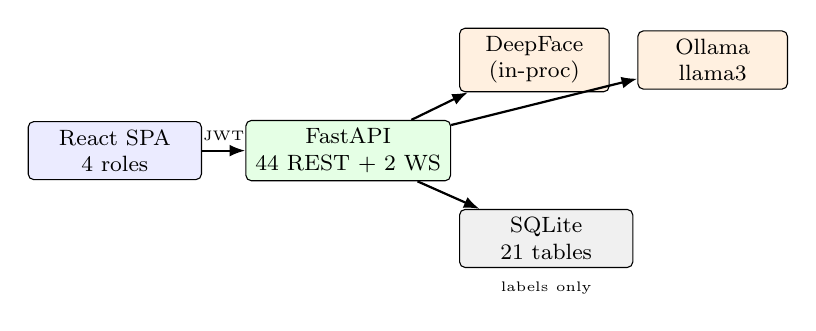
\begin{tikzpicture}[
  font=\footnotesize,
  box/.style={draw, rounded corners=2pt, align=center, minimum height=0.65cm, inner sep=3pt},
  arr/.style={-{Latex[length=2mm]}, thick}
]
\node[box, fill=blue!8, minimum width=2.2cm] (ui) {React SPA\\4 roles};
\node[box, fill=green!10, minimum width=2.6cm, right=0.55cm of ui] (api) {FastAPI\\44 REST + 2 WS};
\node[box, fill=orange!12, minimum width=1.9cm, above right=0.35cm and 0.1cm of api] (df) {DeepFace\\(in-proc)};
\node[box, fill=orange!12, minimum width=1.9cm, right=0.35cm of df] (oll) {Ollama\\llama3};
\node[box, fill=gray!12, minimum width=2.2cm, below right=0.35cm and 0.1cm of api] (db) {SQLite\\21 tables};
\draw[arr] (ui) -- node[above]{\tiny JWT} (api);
\draw[arr] (api) -- (df);
\draw[arr] (api) -- (oll);
\draw[arr] (api) -- (db);
\node[below=0.05cm of db, align=center, text width=2.4cm] {\tiny labels only};
\end{tikzpicture}}
\caption{Local-first SyNAPSE architecture. Webcam frames are processed in memory; only derived affect labels persist.}
\label{fig:arch}
\end{figure}

\subsection{Session and Alert Pipeline}
Fig.~\ref{fig:pipe} summarizes the student path. Emotion capture is \textbf{user-triggered} (not continuous polling). \texttt{POST /api/emotion/detect} resizes frames (max 320\,px), runs DeepFace with OpenCV backend under a threading lock, writes \texttt{EmotionLog}, evaluates \texttt{maybe\_create\_emotion\_alert} when emotion $\in$ \{sad, angry, fear, disgust, \ldots\} and confidence $\geq 0.35$, then broadcasts on \texttt{/ws/alerts}. \texttt{POST /api/cards/generate} queries Ollama (120\,s timeout) and assembles 16 cards.

\begin{figure}[!t]
\centering
\resizebox{\columnwidth}{!}{%
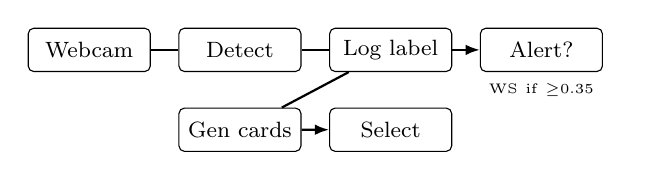
\begin{tikzpicture}[
  font=\footnotesize,
  proc/.style={draw, rounded corners=2pt, align=center, minimum width=1.55cm, minimum height=0.55cm},
  arr/.style={-{Latex[length=1.8mm]}, thick}
]
\node[proc] (cam) {Webcam};
\node[proc, right=0.35cm of cam] (det) {Detect};
\node[proc, right=0.35cm of det] (log) {Log label};
\node[proc, right=0.35cm of log] (alt) {Alert?};
\node[proc, below=0.45cm of det] (gen) {Gen cards};
\node[proc, right=0.35cm of gen] (sel) {Select};
\draw[arr] (cam)--(det)--(log)--(alt);
\draw[arr] (log)--(gen)--(sel);
\node[below=0.02cm of alt, text width=2.1cm, align=center] {\tiny WS if $\geq$0.35};
\end{tikzpicture}}
\caption{On-demand emotion detection, zero-retention logging, optional WebSocket alert, and adaptive card generation.}
\label{fig:pipe}
\end{figure}

\subsection{Technology Stack}
Table~\ref{tab:stack} summarizes implementation choices. Default Ollama model is \texttt{llama3} (\texttt{OLLAMA\_MODEL} override supported)~\cite{ollama2024,meta2024}.

\begin{table}[!t]
\centering
\caption{Technology stack (prototype v1.0.0).}
\label{tab:stack}
\small
\begin{tabular}{@{}ll@{}}
\toprule
\textbf{Layer} & \textbf{Choice} \\
\midrule
Frontend & React 18, Vite, TailwindCSS \\
API & FastAPI, Uvicorn, python-jose JWT \\
Persistence & SQLite, SQLAlchemy (21 tables) \\
Expression & DeepFace, OpenCV, 320\,px cap \\
LLM & Ollama \texttt{llama3}, JSON + fallback \\
Reports & ReportLab A4 PDFs (KHDA/SEND) \\
Realtime & \texttt{/ws/session/\{id\}}, \texttt{/ws/alerts} \\
\bottomrule
\end{tabular}
\end{table}

\section{Implementation}
\subsection{API Surface and RBAC}
SyNAPSE exposes \textbf{44 REST endpoints} and \textbf{two WebSockets} (46 rows in \texttt{functional\_test\_coverage.csv}). Table~\ref{tab:api} summarizes router prefixes. Roles: \texttt{student}, \texttt{teacher}, \texttt{caregiver}, \texttt{send\_officer}. Demo seed users (\texttt{demo1234}) include Ahmed (student), Ms.\ Sarah Ahmed (teacher), Dr.\ Khalid Al Mansoori (SEND officer), and Fatima Al Rashidi (caregiver).

\begin{table}[!t]
\centering
\caption{REST endpoint counts by router.}
\label{tab:api}
\small
\begin{tabular}{@{}lcr@{}}
\toprule
\textbf{Router} & \textbf{Prefix} & \textbf{\#} \\
\midrule
auth & \texttt{/auth} & 3 \\
children & \texttt{/api/children} & 4 \\
sessions & \texttt{/api/sessions} & 5 \\
emotion & \texttt{/api/emotion} & 1 \\
cards & \texttt{/api/cards} & 2 \\
assessment & \texttt{/api/assessments} & 6 \\
reports & \texttt{/api/reports} & 8 \\
send & \texttt{/api/send} & 2 \\
teacher & \texttt{/teacher} & 9 \\
alerts & \texttt{/api/alerts} & 2 \\
support & \texttt{/api/support} & 1 \\
main & \texttt{/}, \texttt{/health} & 2 \\
\midrule
\multicolumn{2}{l}{\textbf{REST total}} & \textbf{44} \\
\multicolumn{2}{l}{WebSockets} & 2 \\
\bottomrule
\end{tabular}
\end{table}

\subsection{Database Schema}
Twenty-one SQLAlchemy tables support AAC sessions, assessments, and wellbeing features: \texttt{users}, \texttt{children}, \texttt{sessions}, \texttt{emotion\_logs}, \texttt{card\_selections}, \texttt{emotion\_alerts}, \texttt{assessments}, \texttt{routine\_templates}, \texttt{routine\_steps}, \texttt{sensory\_profiles}, \texttt{calm\_corner\_sessions}, \texttt{break\_activities}, \texttt{break\_logs}, \texttt{reward\_goals}, \texttt{reward\_events}, \texttt{badges}, \texttt{video\_models}, \texttt{self\_reports}, \texttt{display\_preferences}, \texttt{shared\_notes}, \texttt{pre\_event\_plans}.

\subsection{AAC Card Model}
\texttt{cards\_service.py} returns exactly 16 cards: eight bilingual core symbols (\emph{I want}/\emph{أريد}, \emph{Stop}/\emph{توقف}, \ldots), four emotion-specific cards keyed to the detected label, and four topic slots filled by LLM output or rule templates. Topics in benchmarks: \texttt{school}, \texttt{home}, \texttt{play}, \texttt{food}, \texttt{feelings}, \texttt{body}. Card selections persist with \texttt{emotion\_at\_selection}.

\subsection{SEND Assessment and Reporting}
SEND officers create six-phase assessments, attach observational notes, and complete workflows invoking \texttt{pdf\_service} (ReportLab). \texttt{reports\_router} serves per-child history, session PDF generation, and KHDA-style school reports---endpoints implicated in four RBAC failures before fixes (Section~\ref{sec:rbac}).

\subsection{Privacy and Ethics}
Aligned with IEEE ethically aligned design~\cite{ieee2019,unicef2021}: local processing, no frame persistence, role-scoped queries, and caregiver alert cooldown (45\,s). Arabic UI strings exist; formal RTL usability review was not conducted.

\section{Evaluation Methodology}
Eight integration-benchmark scripts in \texttt{synapse/tests/evaluation/} write CSVs to \texttt{results/}. A starter \texttt{pytest} suite (13 tests: auth, RBAC, emotion pipeline) lives in \texttt{backend/tests/}. \texttt{functional\_test\_coverage.csv} marks only 3/46 endpoints with direct \texttt{has\_test=True}.

\textbf{Hardware.} Single developer workstation, CPU inference, local Ollama; benchmarks run 2026-09-01 UTC. \textbf{Threats to validity.} Seeded demo data, no child participants; LLM cold-start outliers inflate mean latency; emotion pilot uses 12 FER-2013 crops with only three ground-truth classes after \texttt{embedded\_fer2013.json} corruption.

\section{Results}
\subsection{Latency and Reliability}
Table~\ref{tab:bench} reports statistics from benchmark CSVs. LLM latency is \textbf{bimodal}: four runs exceed 20\,s (cold-start) while steady-state runs cluster near 5--9\,s.

\begin{table}[!t]
\centering
\caption{Performance benchmarks (\texttt{results/}, 2026-09-01).}
\label{tab:bench}
\small
\begin{tabular}{@{}lrrrr@{}}
\toprule
\textbf{Metric} & \textbf{$n$} & \textbf{Mean} & \textbf{Med.} & \textbf{Max} \\
\midrule
PDF gen (s) & 30 & 0.317 & 0.199 & 1.010 \\
LLM cards (s) & 36 & 10.56 & 7.36 & 36.18 \\
WS alert (s) & 30 & 0.724 & 0.698 & 1.233 \\
LLM fallback & 120 & \multicolumn{3}{c}{22 events (18.3\%), all malformed JSON} \\
\bottomrule
\end{tabular}
\end{table}

\subsection{Role-Based Access Control}
\label{sec:rbac}
We executed 168 authenticated requests (four roles $\times$ 42 protected patterns). \textbf{168/168 (100\%)} matched expected policy after fixes in \texttt{reports\_router.py} (\texttt{\_authorize\_session\_report\_access}) and \texttt{teacher\_router.py} (\texttt{readiness\_status} shadowing bug). Prior failures: four incorrect 403s on session report/PDF routes; six teacher routes returning status~0 instead of 403.

\subsection{Emotion Integration Pilot}
\texttt{bench\_emotion\_detection\_accuracy.py} evaluated 12 FER-2013-derived crops. Current fixtures contain only angry (5), disgust (5), and fear (2) after \texttt{embedded\_fer2013.json} corruption; happy, neutral, sad, and surprise classes are absent. Legacy placeholder images (colored rectangles, no facial features) produced 0/12 accuracy with spurious sad/fear bias. After FER-aware preprocessing in \texttt{deepface\_service.py} (histogram equalization, 224\,px upscale, placeholder rejection), \textbf{top-1 accuracy = 5/12 (41.7\%)} with \textbf{macro-F1 = 0.500} (per-class F1 over present ground-truth labels). Table~\ref{tab:emotion} lists per-frame outcomes.

\begin{table}[!t]
\centering
\caption{Per-frame emotion pilot results (\texttt{emotion\_detection\_accuracy.csv}).}
\label{tab:emotion}
\scriptsize
\begin{tabular}{@{}lllcc@{}}
\toprule
\textbf{Frame} & \textbf{Ground truth} & \textbf{Predicted} & \textbf{Conf.} & \textbf{OK} \\
\midrule
f001 & angry & fear & 0.72 & $\times$ \\
f002 & angry & neutral & 0.90 & $\times$ \\
f003 & angry & angry & 0.95 & $\checkmark$ \\
f004 & angry & angry & 1.00 & $\checkmark$ \\
f005 & angry & sad & 0.40 & $\times$ \\
f006 & disgust & sad & 0.98 & $\times$ \\
f007 & disgust & angry & 0.53 & $\times$ \\
f008 & disgust & fear & 1.00 & $\times$ \\
f009 & disgust & disgust & 0.99 & $\checkmark$ \\
f010 & disgust & neutral & 0.59 & $\times$ \\
f011 & fear & fear & 0.74 & $\checkmark$ \\
f012 & fear & fear & 0.96 & $\checkmark$ \\
\bottomrule
\end{tabular}
\end{table}

\subsection{Alert Threshold Sensitivity}
Table~\ref{tab:alert} summarizes \texttt{bench\_alert\_precision\_recall.py} on the same 12 frames (all labeled distress). Production uses \texttt{MIN\_ALERT\_CONFIDENCE = 0.35}.

\begin{table}[!t]
\centering
\caption{Alert precision/recall by threshold ($n{=}12$ frames).}
\label{tab:alert}
\small
\begin{tabular}{@{}cccccc@{}}
\toprule
\textbf{Thr.} & \textbf{TP} & \textbf{FP} & \textbf{FN} & \textbf{Prec.} & \textbf{Rec.} \\
\midrule
0.25 & 10 & 0 & 2 & 1.00 & 0.833 \\
0.35 & 10 & 0 & 2 & 1.00 & 0.833 \\
0.45 & 9 & 0 & 3 & 1.00 & 0.750 \\
\bottomrule
\end{tabular}
\end{table}

Missed alerts at 0.35: frames f002 and f010 (predicted neutral, below cautious threshold).

\section{Discussion}
\textbf{Validated strengths.} Sub-second median WebSocket delivery supports timely caregiver notification. PDF generation remains interactive. Rule-based LLM fallback yields usable grids despite JSON fragility. RBAC enforces school-style separation at 168/168 after ACL fixes.

\textbf{Open risks.} Emotion pilot is partial-class and $n{=}12$; angry/disgust confusion persists. Restore balanced \texttt{embedded\_fer2013.json} (2 crops $\times$ 6 classes) before efficacy claims. LLM tail latency warrants warm-up or smaller quantized models.

\textbf{ICAMAC fit.} Primary: S4.1 (architecture), S4.16 (benchmarking), S3.19 (ethics), S3.18 (NLP/LLM). S3.13 applies as \emph{integration}, not novel FER. We do not claim cybersecurity (S1) or metaverse (S2) contributions.

\textbf{AI disclosure.} Manuscript structure was drafted with AI writing assistance; all quantitative claims were verified against source code and CSV benchmarks, per IEEE/ICAMAC policy.

\section{Conclusion}
SyNAPSE demonstrates a reproducibly measured, local-first, emotion-aware AAC architecture integrating DeepFace, Ollama Llama~3, FastAPI, and multi-stakeholder school workflows. Verified metrics cover PDF/LLM/WebSocket latency, 18.3\% LLM fallback, 100\% RBAC correctness, 13 pytest tests, and a preliminary FER integration pilot (41.7\% on partial fixtures). Next steps: restore balanced emotion fixtures, expand evaluation ($n{\geq}50$), and broaden automated test coverage.

\balance
\begin{thebibliography}{15}
\bibitem{asha2023} American Speech-Language-Hearing Association, ``Augmentative and Alternative Communication (AAC),'' ASHA Practice Portal, 2023.
\bibitem{monkaresi2017} S. Monkaresi \emph{et al.}, ``Automatic detection of engagement using video-based estimation of facial expressions and heart rate,'' \emph{IEEE Trans. Affect. Comput.}, vol.~8, no.~1, pp.~15--28, 2017.
\bibitem{ekman1978} P. Ekman and W. V. Friesen, \emph{Facial Action Coding System}. Palo Alto, CA: Consulting Psychologists Press, 1978.
\bibitem{goodfellow2013} I. J. Goodfellow \emph{et al.}, ``Challenges in representation learning: Facial expression recognition challenge,'' 2013.
\bibitem{serengil2020} S. I. Serengil and A. Ozpinar, ``LightFace: A hybrid deep face recognition framework,'' in \emph{Proc. ASYU}, 2020.
\bibitem{rowland2024} C. Rowland \emph{et al.}, \emph{Communication Matrix}, Oregon Health \& Science Univ., 2024.
\bibitem{aslan2021} S. Aslan, S. Koushik, and M. Chetouani, ``Automatic recognition of autism based on machine learning,'' in \emph{Proc. IEEE ICASSP}, 2021.
\bibitem{ieee2019} IEEE, \emph{Ethically Aligned Design}, 2019.
\bibitem{unicef2021} UNICEF, \emph{Policy Guidance on AI for Children}, ver.~2.0, 2021.
\bibitem{khda2017} Knowledge and Human Development Authority, Dubai inclusive education policy framework, 2017.
\bibitem{who2022} World Health Organization, \emph{Global Report on Assistive Technology}, Geneva, 2022.
\bibitem{ramirez2018} S. Ram\'irez, ``FastAPI,'' 2018.
\bibitem{react2024} React Team, ``React,'' 2024.
\bibitem{ollama2024} Ollama Project, ``Model library,'' 2024.
\bibitem{meta2024} Meta AI, ``Llama~3 model card,'' 2024.
\end{thebibliography}

\end{document}
